\documentclass[conference]{IEEEtran}

\ifCLASSINFOpdf
  % \usepackage[pdftex]{graphicx}
  % declare the path(s) where your graphic files are
  % \graphicspath{{../pdf/}{../jpeg/}}
  % and their extensions so you won't have to specify these with
  % every instance of \includegraphics
  % \DeclareGraphicsExtensions{.pdf,.jpeg,.png}
\else
  % or other class option (dvipsone, dvipdf, if not using dvips). graphicx
  % will default to the driver specified in the system graphics.cfg if no
  % driver is specified.
   \usepackage[dvips]{graphicx}
  % declare the path(s) where your graphic files are
  % \graphicspath{{../eps/}}
  % and their extensions so you won't have to specify these with
  % every instance of \includegraphics
  % \DeclareGraphicsExtensions{.eps}
\fi

% correct bad hyphenation here
\hyphenation{op-tical net-works semi-conduc-tor}
\usepackage{graphicx}
\usepackage{pdfpages}
\usepackage[cmex10]{amsmath}
\usepackage{enumerate}
\usepackage{epstopdf}


% for annotation
\usepackage{xcolor}
\newcommand{\red}[1] {{\textcolor{red}{#1}}}
\usepackage[normalem]{ulem}
\newcommand{\del}[1] {\sout{#1}}

\begin{document}
%
% paper title
% can use linebreaks \\ within to get better formatting as desired
\title{An explicit congestion notification transport control mechanism for NDN}

\author{\IEEEauthorblockN{Jianer Zhou\IEEEauthorrefmark{1}\IEEEauthorrefmark{2},
Qinghua Wu\IEEEauthorrefmark{1}\IEEEauthorrefmark{2},
Yonggong Wang\IEEEauthorrefmark{1}\IEEEauthorrefmark{2},
Zhenyu Li\IEEEauthorrefmark{1},
Gaogang Xie\IEEEauthorrefmark{1}}
\IEEEauthorblockA{\IEEEauthorrefmark{1}Institute of Computing Technology, Chinese Academy of Sciences, Beijing, China}
\IEEEauthorblockA{\IEEEauthorrefmark{2}University of Chinese Academy of Sciences, Beijing, China}
\{zhoujianer, wuqinghua, wangyonggong, zyli, xie\}@ict.ac.cn}


% make the title area
\maketitle


\begin{abstract}
%\boldmath
Named Data Network(NDN) is a new Internet architecture. Its change of the network layer also sheds light on the transport layer. The Data which comes back along the same path of the Interest natively acts as a barrier of the Explicit Congestion Notification (ECN) information to receiver.  Avoiding a congesting path can be achieved by adaptive forwarding which is a main feature of the NDN data plane. In this paper we implement an ECN transport mechanism in NDN, using the Data to carry ECN information. And we make use of network-wide information of the SDN controller  to design smart forwarding mechanism. Our simulations in ndnSim show that the ECN transport mechanism outperform TCP-style NDN transport mechanisms in link utilization, packet dropping and flow complete time. The network-view information of the SDN controller can optimize the adaptive forwarding in NDN. By joining the ECN transport mechanism and smart forwarding, the total flow complete time can be reduced.

\emph{Index Terms}-NDN, Transport mechanism, ECN, Congestion control, Adaptive forwarding
\end{abstract}

\IEEEpeerreviewmaketitle

%!TEX root = main.tex

\section{Introduction}
% no \IEEEPARstart

% Internet consumers now care more about ``what" they can get from network. However TCP/IP, the network architecture of Internet, is initially designed based on the principle of ``where" to connect the users. This mismatch between the user-demand and network-principle makes the network difficult to satisfy the users. To overcome this, some clean-state network architectures have been proposed. NDN is one of such clean-state architecture\cite{NDN}. In NDN, consumers just send Interest into the network, and the network will return the corresponding Data to it. The consumers are unnecessary to care about where to get the Data.

% As the NDN network layer is based on best-effort transmit model, congestion and dropping packets are still possible. Transport control is still necessary to guarantee effective transfer. Some TCP-style transport control mechanisms have been proposed for NDN, such ICP\cite{ICP}, CCTCP\cite{CCTCP} and HR-ICP\cite{shape}. However these TCP-style transport mechanisms in NDN still have the same problems as TCP/IP, such as low link utilization and high packets dropping rate. Explicit Congestion Notification(ECN) is a promise way to achieve high link utilization\cite{XCP} . Adaptive forwarding is a new feature of the NDN\cite{Adaptive}. Adaptive forwarding let router choose a suitable path according the network situation. If the router senses the link has been congested, then it can choose another path. It is completely different with TCP/IP. In TCP/IP the forwarding process is strictly followed the route table. By the adaptive forwarding, router can deal with the network congestion quickly.

% But by now, as what we have known, no ECN-style congestion mechanism has been proposed in NDN and there is little research about the congestion avoiding mechanism making use of the adaptive forwarding. In this paper we use the Data(which comes back along the same path with Interest) to carry the ECN information, and design an ECN transport mechanism for NDN. We also make use of the SDN's network-wide information to design a smart forwarding mechanism. Joining the ECN and smart forwarding mechanism, we can not only improve single link bandwidth utilization but also the whole network resource utilization. Summary, our main contributions are:

% \begin{enumerate}
% \item[1.] First achieve an ECN transport mechanism in NDN.
% \item[2.] First use SDN-style control information to design smart forwarding mechanism to ultimately use the whole network resource.
% \item[3.] Packet-level simulation shows that joining ECN and smart forwarding in NDN can improve link utilization and total flow complete time.
% \end{enumerate}

Internet consumers typically care more about \emph{what} information they want, instead of \emph{where} it is located. However, the Internet architecture is initially designed for point-to-point communication. This mismatch between user demand and network infrastructure makes Internet applications struggling with the gap between where and what. Several clean slate network architectures have been proposed to address this problem. Among those proposals, NDN\cite{NDN} assigns each data a unique name for addressing and caching, which is compatible with Internet demand and exhilarate information dissemination greatly. 

As NDN adopts simple best-effort packet transport between neighboring NDN nodes, congestion might occur and packets could be dropped due to congestion. Therefore transport control is essential for effective and efficient data transmission. Some TCP-style transport control mechanisms in NDN have been proposed, such as ICP\cite{ICP}, CCTCP\cite{CCTCP} and HR-ICP\cite{shape}. These TCP-style proposals still suffer from the same problems as that in TCP, e.g. low link utilization, high packet dropping rate. Explicit Congestion Notification (ECN) is a promising technique to achieve high link utilization\cite{XCP}. Adaptive forwarding\cite{Adaptive} in NDN is proposed which lets router adaptively select forwarding interface among the multiple available ones according to network condition. Different from TCP/IP in which forwarding interfaces are determined statically, adaptive forwarding could react to congested links and bypass them quickly.

As far as we know, there's still no ECN-style congestion mechanism proposed for NDN and little research about congestion avoidance mechanism by utilizing adaptive forwarding has been investigated. In this paper, by utilizing the feature in NDN that there's one-to-one mapping of Interest-Data and Data is forwarded back along exactly the path Interest is transmitted, in Data packet we introduce an ECN field, which contains ECN information to notify consumer or down-stream routers to adapt their transmission rate. What's more, we also exploit the power of network-wide information by SDN\cite{SDN} to design a smart \red{forwarding} mechanism. By combining ECN and smart forwarding mechanism, we could not only improve bandwidth utilization on single links but also the resource utilization in the whole network. In summary, our main contribution are:

\begin{enumerate}
	\item[1.] We first propose an ECN-based transport mechanism in NDN.
	\item[2.] We are the first to utilize SDN technique to design smart forwarding mechanism to fully exploit the resource in the whole network.
	\item[3.] Packet-level simulation shows that joint ECN and smart forwarding in NDN could improve link utilization and total Flow Complete Time (FCT).
\end{enumerate}

The rest of the paper is organized as followed: Sec. \ref{sec:related} discusses related works. In Sec. \ref{sec:bg} we introduce the NDN's feature which we utilize to design our transport mechanism. In Sec. \ref{sec:rationale} we discuss the design rationale. Sec. \ref{sec:design} introduces the ECN congestion mechanism and the smart forwarding. In Sec. \ref{sec:simulation}, we demonstrate the effectiveness of our mechanism. Finally Sec. \ref{sec:conclude} concludes the paper.

%!TEX root = main.tex

\section{Related work}

\label{sec:related}

% Two kinds of congestion control mechanisms have been widely studied in the traditional network transport layer.

% TCP-style. TCP-style mechanisms are widely used nowadays.  Every sender maintains a sending window. The sending window will additively increase if the RTT is below an estimated value, otherwise window will multiplicatively decrease\cite{TCP}. TCP-style mechanism is very easy to implement, just on the host. But the utilization is low in high bandwidth-delay network because the slow start principle and it is unfair when long flow competes with short flow.

% ECN-style. ECN-style mechanism uses ECN information to sense the condition of the network, such as XCP\cite{XCP}, RCP\cite{RCP}. The senders react its sending rate according the ECN information. Compared with TCP-style, who use implicit congestion information, ECN-style can effectively use the network resource and achieve fairness. Although our Interest sending rate's design principle is similar with RCP, our design process is different. In this paper we use \emph{R(t)} to control the receiver's sending rate, but RCP use the \emph{R(t)} to control the sender's packet sending rate. We also have to consider the size of Data, and in RCP the packet's size has not relationship with the design process.

Congestion control mechanisms in TCP/IP network can be grouped into two categories:

\emph{Congestion Window} Congestion window mechanism is widely deployed nowadays. Each end in the communication maintains a congestion window, which will additively increase if the RTT is below the estimation value, otherwise multiplicatively decrease, known as AIMD\cite{TCP}. Congestion window mechanism is easy to deploy since it only requires modification in end hosts. However, congestion window results to low utilization in high bandwidth-delay networks because of the slow start function. Moreover, it results in unfairness for short flows when mixed with long flows.

\emph{Explicit Congestion Notification (ECN)} ECN mechanism notifies network condition by explicit information, such as in XCP\cite{XCP}, RCP\cite{RCP}. Router generates ECN information according to network condition and send it to end host. End host adjusts its transmission rate according to the ECN information it has received. Compared with implicit congestion information in TCP, ECN can effectively utilize network resource and achieve fairness. However, RCP use congestion information to control server's transmission rate, which is contrary to the consumer-driven nature in NDN. Besides, RCP does not consider the impact of Data size on the estimation of flow size, which is also essential in congestion control in NDN.


% Those works above failed to achieve considerable performance in congestion control in NDN because they do not utilize its specific property, such as consumer-driven, one-to-one mapping between Interest and Data.

Some transport mechanisms have been proposed for NDN. Most of them is TCP-style. Some researchers use NDN's features, such as the NACK, to improve the TCP-style mechanism.

\emph{Receiver driven TCP-style} Different with TCP/IP's push principle, NDN is a receiver-driven network architecture. In NDN, receivers control transmission rate by adapting the rate of sending Interest. Thus, most of proposed transport mechanisms in NDN are receiver-driven. Receiver adjust its Interest sending rate according to the RTT of the coming back Data, using the AIMD and slow start principle. Contug et al.\cite{Contug} propose transport mechanism in NDN which mixes receiver-driven mechanism and the basic principles in TCP. It just changes the congestion-controller from sender to receiver. In\cite{Flow}, Sara et al. separate the traffic into different flows according to name prefix. Each flow uses TCP-like mechanism to control the congestion. Routers fairly allocate the bandwidth to each flow, and use optimal buffer algorithm to improve the performance. In NDN, due to in-network cache, content can be retrieved from different providers or routers. Different locations of content may result in multipath in transport layer. In \cite{Multipath}, Givonaan et al. deal with the multipath problem in NDN, using similar way as the MTCP.

\emph{Interest NACK} In NDN an Interest is much smaller than a Data. Intuitively, it is much more ``resource-saving'' if we drop Interest instead of Data when congestion happens. In HR-ICP\cite{shape}, routers shape the Interest hop-by-hop to handle or prevent congestion. Each router shapes Interest just by itself, according the bandwidth it can supply to incoming Data. In \cite{improveshape} Wang et al. improve the Interest shaping mechanism as follows. Once an Interest is shaped, router sends NACK back to the receiver to inform that congestion has occurred. Although NACK implies congestion, it does not inform how severe the congestion is. The receiver simply cuts half of the Interest sending window when it receives NACK, which will reduce the link utilization significantly as in TCP. Furthermore, the shaping mechanism, no matter Interest or Data will cause retransmission, which will increase the flow complete time.

To fit the pull principle of NDN, all of these above mechanisms use the receiver to deal with congestion. But they still follow the TCP's slow start and AIMD implicit congestion principle. They also have the low utilization and unfairness problems, similar with TCP\cite{NDNanalysis}.

%!TEX root = main.tex

\section{Background}
We recall come features of NDN that we will use to design our transport mechanism. The full description of NDN can be found in NDN paper\cite{NDN}\cite{Adaptive}.

Data feedback. In NDN, consumers send Interest to request Data. The router uses Content Store, Pending Interest Table(PIT) and Forwarding Information Base(FIB) to return , record and forward the Interest respectively. For every consumer, one Interest pull back exactly one Data. As the PIT maintains every Interest's state, such as the coming and leaving entry, the Data will come back along exactly the same path with Interest. Such ``same path" feedback let the Data natively act as carrier to bring back the ECN information to consumers.

Adaptive forwarding. Adaptive forwarding is a main feature of NDN data plain. In TCP/IP, forwarding table completely follows the route table without any adaptability, and there is just one path to the destination in the route table. However in NDN, during the forwarding process, router can adaptively choose a forwarding interface from several available paths according the network situation. In \cite{Adaptive} Cheng, etc. make use of the adaptive forwarding mechanism to design a hop-by-hop congestion control mechanism. Routers adaptively forward the Interest to another interface (if available) when it detects that the next hop has been congested. Such adaptive forwarding way helps the network solve congestion much easier than the route assistant congestion in TCP/IP, because the route-assistant congestion mechanism needs the help of route protocol\cite{selfish}. However such just one hop detection is not enough if the congestion happens on later link, because the one hop detection cannot sense it.  SDN-style solution can get the network-wide information. And such network-wide information is a promise way to overcome the limit of the just one hop information.

%!TEX root = main.tex

\section{Design rationale}

\label{sec:rationale}

% When we initially think about the transport control mechanism in new network architecture, the first question is who dominant and should be responsible for the congestion control? In TCP/IP, as its push principle, it is the senders who deal with the network congestion by changing the packet sending window. Under the pull nature of NDN, it is obviously that the receivers should be responsible for the network congestion. The one-Interest one-Data principle makes it possible to control the network traffic through the control of Interest sending rate. Such control congestion is called receiver-driven transport mechanism\cite{Contug}. Our design also follows the receiver-driven principle.

% If several flows share one link, it is ideal that the link bandwidth is ultimately used and at the same time fairly shared by all the flows. ECN information reflects the network resource situation such as that the available bandwidth and flow number of the path. By the ECN information, receivers can adjust its Interest sending rate to ultimately use the bandwidth and achieve fairness. So our first design goal is to use the ECN information to control the receiver's Interest sending rate.

% By controlling the receiver's Interest sending rate, we can perhaps ultimately use the link bandwidth and avoid congestion. But if all the flows choose a path that goes through the same bottleneck, even we can ultimately use the link bandwidth, the flow complete time can be low, because too many flows share the same bottleneck. So if there are several paths available for the flows, how can we choose different paths for different flows that minimum all the flows' complete time? Our second design goal is to design a smart forwarding mechanism that minimum flow complete time.
 
% In TCP/IP, the route path is single path, and the forwarding process is strictly follows the route path. Choosing path adaptively is very difficult. However, in NDN, the adaptive forwarding makes it possible. Take the mesh network topology in Fig. \ref{fig-topology}. as example. A flow goes through router5. The flow has two available paths to get the data from provider. Router5 can easily measure the congestion condition at the link1 (between router5-7) and link2 (between router5-8). If the router senses that link1 is much more congested than link2 then the router can adaptively forward the flow to link2. By such adaptive forwarding, the network resource can be effectively used and reduce the flow complete time.
 
% But such just one hop measure way is very limited. Take the same situation as example. The true bottleneck happens on link3 (between router10-13). But the router5 can measure just one hop situation, it cannot sense the true bottleneck is on the link3, so it will still forward the interest to link2. The wrong forwarding decision will add more burdens to link3, and reduce the flow complete time of all the flows.
 
% The SDN-style controller can get the whole network information. We will introduce the SDN's network-wide information to overcome the ��limited information�� problem. By the network-view information, the Interest can be forwarded to the best path. The whole network bandwidth utilization and total flow complete time can be improved.

When we to design transport control mechanism for a new network architecture, the first question is which entity should be responsible for the congestion control. In TCP/IP, as its push principle, it is the sender who deals with network congestion by adjusting the packet sending window. Under the pull nature of NDN, it is obvious that receivers should be responsible for the network congestion. The one-to-one mapping of Interest-Data makes it possible to control the network traffic through the control of Interest sending rate. Such control congestion is called receiver-driven transport mechanism\cite{Contug}. Our design also follows the receiver-driven principle.

If multiple flows are transmitted through one link, it is ideal that the link bandwidth is fully utilized and at the same time fairly shared by all the flows. ECN information reflects the network resource situation such as the available bandwidth and the number of flows on the path. According to the ECN information, receiver adjusts its Interest sending rate to fully use the bandwidth and achieve fairness. So our first design goal is to use the ECN information to control the receiver's Interest sending rate.

By controlling receivers' Interest sending rate, we can perhaps fully use the link bandwidth and avoid congestion. But if all the flows choose a path that goes through the same bottleneck, even we can fully use the link bandwidth and achieve fairness, the flow complete time can be very low, because too many flows share the same bottleneck. So if there are several paths available for the flows, how can we allocate the multiple paths to each flow to minimize the total flow complete time? Our second design goal is to design a smart forwarding mechanism that minimizes total flow complete time.

In TCP/IP, only a single path is available for each source destination pair, and the forwarding process strictly follows the single path, thus adaptively selecting alternative path is very difficult. However, in NDN, the adaptive forwarding makes it possible. Taking the mesh network topology in Fig. \ref{fig-topology} for example, a flow goes through $R5$. The flow has two available paths to get the data from provider. Router $R5$ can easily measure the congestion condition at the link1 (between router $R5$ and $R7$) and link2 (between router $R5$ and $R8$). If the router senses that link1 is much more congested than link2 then the router can adaptively forward the flow to link2. By such adaptive forwarding, the network resource can be effectively used and the flow complete time will be reduced.

However, such a one-hop measurement is very limited. Taking the same situation for example, the true bottleneck happens on link3 (between router $R10$ and $R13$). But the router $R5$ can measure just one hop situation, it cannot sense the true bottleneck is on the link3, so it will still forward the interest to link2. The wrong forwarding decision will put more burdens to link3, and increase the flow complete time of all the flows.

The SDN-style controller can get the whole network information. We will introduce the SDN's network-wide information to overcome the ``limited information'' problem. By the network-view information, the Interest can be forwarded to the best path. The whole network bandwidth utilization will be improved and total flow complete time can be reduced.

%!TEX root = main.tex
\section{Design}

\label{sec:design}

To achieve the two goals above, our design divided into three parts. First we design the ECN Interest sending rate on the receiver. Second we design a smart forwarding mechanism and at last we analysis the convergence and stability of the system.

\subsection{ECN Interest sending rate}
Our motivation is to send Interest at a maximum rate that the path can handle the corresponding coming back Data without dropping. To achieve this, every router on the path should calculates each flow's maximum Interest sending rate that it can handle, without causing congestion. We define such maximum rate as $R(t)$.

Fig.~\ref{fig-header} shows the Interest and Data ECN header. The ECN header contains the explicit congestion notification information on the path. The Interest carries the RTT(Round Trip Time) of the flow. The RTT is defined as the interval between the time receiver sends an Interest to the time it receives the corresponding Data. In our design, RTT is used to determine the updating interval of $R(t)$. The provider copied the Interest's RTT to Data when it send back the Data, and the routers do not change it along the path. The router compares the $R(t)$ that is recorded in the Data with its own $R(t)$. If the router's rate is smaller, it replaces it. By this way, the coming back Data carries the minimum $R(t)$ of all the routers along the path. As the Data comes back along the same path of the Interest, the rate on the Data also reflects the path of the Interest. Each receiver sends its Interest according the $R(t)$ it receives last Data.

\begin{figure}[t]
	\centering
	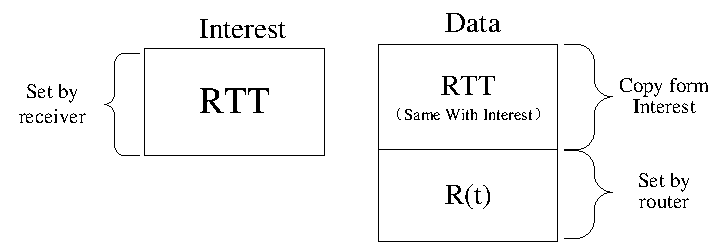
\includegraphics[width=2.5in]{header-ndn.pdf}
	\caption{Explicit congestion notification header for Interest and Data.}
	\label{fig-header}
\end{figure}

Suppose we know how many flows going through a link, and we want to share its bandwidth with all the flows, then $R(t)$ can be determined as follows:
\begin{equation}
	\label{eq:rt}
	R(t)=\frac{C}{Flow_{num}*Size_{d}} \enspace .
\end{equation}
In the equation, $Size_{d}$ is the size of incoming Data, $C$ is the bandwidth of the link, $Flow_{num}$ is the number of flows on the link. Eq.~\ref{eq:rt} is the ideal situation. When the network condition changes, such as a new flow is added, $R(t)$ should be updated. To make the update process reasonable and let the system enter stable situation, Eq.~\ref{eq:rt} should be improved as:
\begin{equation}
	\label{eq:updated_rt}
	R(t)=R(t-RTT_{avg})+\frac{\alpha(C-S(t))-\beta\frac{Q(t)}{RTT_{avg}}}{Flow_{num}*Size_{d}} \enspace
\end{equation}

In the Eq.~\ref{eq:updated_rt}, $R(t)$ is the Interest sending rate that the router assigns to all flows at time $t$, $S(t)$ is the speed of coming back Data, $Q(t)$ is the packets that occupied in the queue at time $t$, $\alpha$ and $\beta$ are the parameters that influence the convergence and performance, $RTT_{avg}$ is the average RTT of all the flows that go through this router. We set $RTT_{avg}$ as the updating interval of $R(t)$.

The definition of $R(t)$ in Eq.~\ref{eq:updated_rt} is explained as follows. The available bandwidth and queue should be fairly shared by all the flows, so the link's available resource is divided by the number of flow. If $(C-S(t))>0$, there are more available bandwidth to be used and the transmission rate of each flow should be increased. Otherwise, the bandwidth has been over used and the sending rate should be reduced. We assume that the packets occupied in the queue should always come to zero. If it is not zero, it means too many Data packets flow into this link, and the Interest sending rate should be reduced. In every $RTT_{avg}$ the router should drain $Q(t)/RTT_{avg}$ Data packets. Because the $R(t)$ is the Interest sending rate, and the available resource is supplied to the Data, so we divide it by the size of Data.

If router tends to make the system converge to stable stage more quickly, it can update $R(t)$ with shorter interval $T$ $(0 < T \leq RTT_{avg})$. Then Eq.~\ref{eq:updated_rt} becomes:
\begin{equation}
	\label{eq:updated_rt3}
	R(t)=R(t-T)+\frac{\frac{T}{RTT_{avg}}\ast(\alpha(C-S(t))-\beta\frac{Q(t)}{RTT_{avg}})}{Flow_{num}*Size_{d}} \enspace .
\end{equation}

Using the prefix of the Interest name to estimate the number of flows traversing through the router will add complexity to the router. In\cite{RCP}, it has been proved that the processor-fair resource allocated way can estimate the flow number by the each flow's sending rate. Processor-fair means routers fairly allocate link bandwidth and queue resource to all flows through this link. So we also use process-fair way to calculate the number of flows that go through this link:
\begin{equation}
	\label{eq:flownum}
	Flow_{num}=\frac{C}{R(t-RTT_{avg})\ast{Size_{d}}} \enspace .
\end{equation}

As we set every flow share the link bandwidth equally, and every flow's rate is the same, it is reasonable to use Eq.~\ref{eq:flownum} to estimate the number of flows. In Sec.~\ref{sec:simulation}, we will evaluate by simulation that the estimation is correctly.
Combining with Eq.~\ref{eq:flownum}, Eq.~\ref{eq:updated_rt3} becomes:
\begin{equation}
	\label{eq:updated_rt5}
	R(t)=R(t-T)[1+\frac{\frac{T}{RTT_{avg}}\ast(\alpha(C-S(t))-\beta\frac{Q(t)}{RTT_{avg}})}{C}] \enspace .
\end{equation}
Many factors may influence the size of Data in NDN, such as the different MTU of different link. So it will be very difficult to exactly measure the size of Data. When we need to use the size of Data to test the accuracy of the flow number estimation, we have to use the historical information to estimate the size of Data. From Eq.~\ref{eq:updated_rt5} we can find that, $R(t)$ does not need to measure the flow number directly and the size of Data. That will greatly simplify the router's calculating process.

\subsection{Smart adaptive forwarding}

In this paper we just control the forwarding process, not the route calculating process. The route algorithm in NDN is on active research. But from the algorithms proposed by now, we can see that the NDN route algorithm is different from TCP/IP\cite{ndnroute}. Traditional route protocol such as OSPF and RIP just have one single path for each destination. But in NDN, Data may have multiple replicas which are distributed in different hosts, so there are multiple paths to get a Data. And even the Data from the same provider may have different available paths. In this paper, we assume the receivers have multiple paths to get a Data, and the routers have known every hop of different paths. The smart adaptive forwarding mechanism we proposed just has relationship with the choose of forwarding interfaces from different paths.

Every router sends its own $R(t)$, the transmit delay and the bandwidth of the next hop to the controller at an interval of $RTT_{avg}$. After several $RTT_{avg}$, the controller can know every router's $R(t)$ and the transmit delay of every hop. We call the information as forwarding-assistant information. The network's route information can also be stored in the controller. By the forwarding-assistant information and route information, we can calculate the best forwarding strategy. The forwarding-assistant and route information stored in the controller is showed in Fig.~\ref{fig-assistant-information}.

\begin{figure}[t]
	\centering
	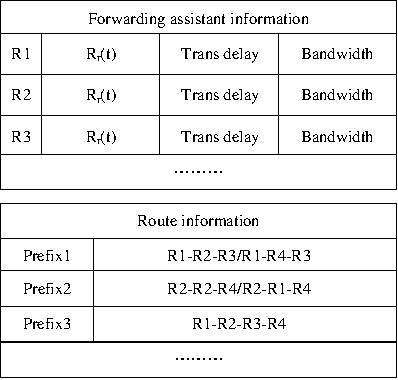
\includegraphics[width=2.5in]{forwarding-assistant-information.pdf}
	\caption{Forwarding assistant and route information stored in the controller.}
	\label{fig-assistant-information}
\end{figure}

Using the Interest sending rate we propose above, the FCT of each flow is:
\begin{equation}
	\label{eq:fct}
	FCT=\frac{Size_{f}}{Size_{d}\ast{R_{b}}}+RTT
\end{equation}
where $Size_{f}$ is the size of the flow, $R_{b}$ is the bottleneck's Interest sending rate, $R_{b}$ can be easily calculated by the forwarding-assistance and route information. Eq.~\ref{eq:fct} means that FCT is the time that the flow goes through the bottleneck plus the RTT of this flow. The RTT of this flow can be calculated by the forwarding-assistant information.

We suppose the $i$-th flow has several available paths. If it chooses path j, then this flow's FCT on path j should be:
\begin{equation}
	\label{eq:fctij}
	FCT_{i,j}=\frac{Size_{f}}{Size_{d}\ast{R^{'}_{b}}}+RTT_j
\end{equation}
where $RTT_j$ is the RTT of flow i if it chooses path j and $R^{'}_{bottleneck}$ is the bottleneck's Interest sending rate on path j.

\begin{equation}
R^{'}_{b}=\frac{C}{Flow_{num}+1} = \frac{C}{C/(R_{b}\ast{Size_{d}})+1}
\end{equation}
For simplicity, we set the value of $Size_{d}$ and $Size_{f}$ as fixed values, and suppose $Size_{data} =Size_{flow}$. So Eq.~\ref{eq:fctij} becomes:
\begin{equation}
FCT_{i,j}=\frac{C/(R_{b}*Size_{d})+1}{C}+RTT_j
\end{equation}

Our design goal is to minimize the Total Flow Complete Time (TFCT) in the network. TFCT is the sum of all the flows' complete time. To achieve our goal we define the objective of the smart forwarding as:
\begin{equation}
	\begin{aligned}
		& \min &&  \sum_{i=0}^{n} FCT_i \\
		& \text{s.t.}  && \text{path } j \text{ is available};\\
		&              && \forall i, P_i \in \{0,1\};\\
		&              && \max \min  R_i \enspace .
	\end{aligned}
\end{equation}
In the equation, $P_i$ is the number of path that flow i chooses. $P_i \in \{0,1\}$ means $Flow_i$ can choose at most one path. $max \ min \ R_i$ means $Flow_{i}$'s Interest sending rate should be maximized. The reason we set $max \ min \ R_i$ is to achieve fairness between different flows. If we do not set $max \ min \ R_i$, some flows may choose a min R to minimum the TFCT, and that will influence this flow's FCT.
% Sacrificing oneself to achieve the goal of minimum TFCT is unfair.

Routers send the updated forwarding-assistance and route information to the controller at the interval of $RTT_{avg}$. The routers send back smart forwarding decision for each flow when it receives the router's updating information. The smart forwarding decision is based on the unit of flow, not the unit of each packet. So the overhead introduced by the controller's help is very limited compared with the whole volume that goes through the router. To timely reflect the change of network information to the controller, routers can change the sending interval, and that will raise the overhead. But the balance between the overhead and the accuracy of updating information can be adaptively controlled.

\subsection{Stability analysis}

The parameters $\alpha$ and $\beta$ influence the stability and convergence of the system. As Eq.~\ref{eq:updated_rt} shows, $\alpha$ influences how the bandwidth is used. If $\alpha$ is large then bandwidth will be occupied quickly. Parameter $\beta$ influences how quickly that the packets in the queue can be drained. Obviously that large $\alpha$ and $\beta$ can help the system to use the resource quickly. But large $\alpha$ and $\beta$ will make the system become unstable, as the network is difficult to convergence.

To choose suitable $\alpha$ and $\beta$ that make the system stable, we test under what $\alpha$ and $\beta$, the flow number can be estimated accurately. Once the flow number of the network can be accurately estimated, the Interest sending rate $R(t)$ can also be estimated accurately, then the system will enter stable stage. So we choose the accuracy of estimating flow number as the stability metrics.

At the beginning, there are 10 flows in the network, and we test whether the flow number can accurately be estimated under different value of $\alpha$ and $\beta$. Fig.~\ref{fig-ab} shows that under such values the flow number can be accurately estimated. Fig.~\ref{fig-abwrong} shows that under these values the estimated flow number change greatly, which means that the system is not stable. From Fig.~\ref{fig-ab}, we can find (0.2,1.5) is the most suitable value to estimate the flow number. Under this value, we test whether the system is still stable when the system changes. We set the number of flows in the network as 5,10,15 and 20 respectively. Fig.~\ref{fig-abflownum} shows that under different situation the flow number can also be accurately estimated when $\alpha=0.2,  \beta=1.5$. That means a fixed value of $\alpha$ and $\beta$ can make the system enter stable stage even when the system's situation changes.

From Fig.~\ref{fig-abwrong}, we find that when $\alpha$ is close to 0.5, the system becomes unstable, and when it gets larger, the system becomes even more unstable. This can be explained as follows. Large $\alpha$ makes the system react too radically to increase $R(t)$ when $(C-S(t))>0$ or decrease $R(t)$ when $(C-S(t))<0$. Radical reaction will make the system difficult to converge. From Fig.~\ref{fig-ab}, we find that when $\alpha < 0.2$, the system will take longer time to accurately estimate the flow number. It is because small $\alpha$ makes the system increase or decrease $R(t)$ conservatively, and that will result in longer time to convergence. When $\beta$ is smaller than 1.5, although the system can be stable, the estimated flow number is not accurate compared with $\beta = 1.5$. It is because small $\beta$ can not drain the packets in the queue quickly enough. And that will result in inaccurate $R(t)$ and flow number.

The key point of the stability analysis is that, for $\alpha$ and $\beta$ we can choose a fixed value to make the system stable. Even when the system changes, such as the flow number, RTT and bandwidth, the fit value can also make the system keep stable. Although now we can not prove the best value by theory, it is possible to choose a suitable value by experimental test. In our simulation, we set $\alpha = 0.2$ and $\beta = 1.5$, according the analysis above.

\begin{figure}[t]
\centering
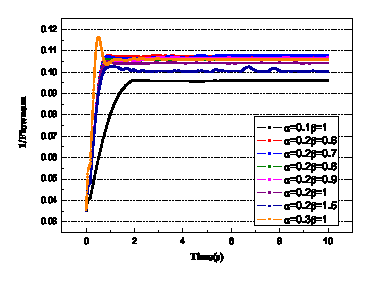
\includegraphics[width=2.5in]{ab-pic-cut.eps}
\caption{Under such $\alpha$ and $\beta$ the flow number can be accurately estimated.}
\label{fig-ab}
\end{figure}

\begin{figure}[t]
\centering
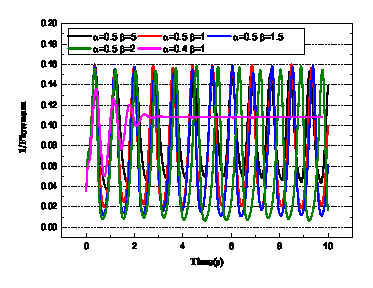
\includegraphics[width=2.5in]{abwrong-pic-cut.eps}
\caption{Under such $\alpha$ and $\beta$ the flow number can not be accurately estimated.}
\label{fig-abwrong}
\end{figure}

\begin{figure}[t]
\centering
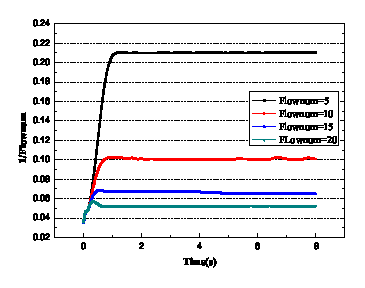
\includegraphics[width=2.5in]{abflownum-pic-cut.eps}
\caption{Stable $\alpha$ and $\beta$ can make the network stable even when network situation changes.}
\label{fig-abflownum}
\end{figure}

%!TEX root = main.tex

\section{Performance Evaluation}

\label{sec:simulation}

In this section, we study the performance of the proposed mechanism using ndnSim\cite{ndnsimnet, ndnsim}.

Our evaluation includes four parts. In the first part we discuss the influence of $\alpha$ and $\beta$ in Eq.~\ref{eq:updated_rt5} to system stability. In the second part we evaluate the flow number estimating process, which we propose in Eq.~\ref{eq:flownum}. In the third part, we evaluate the ECN-based Interest sending(ECN-based) mechanism using the bottleneck network topology. At last we join the Smart forwarding with ECN-based(SECN) and evaluate SECN using the mesh network topology. The evaluation results show the flow number can be estimated accurately. Compared with ICP and ICP-shape, ECN-based mechanism performs better in link utilization, packets dropping and flow complete time. The SECN has better TFCT(Total Flow Complete Time) compared with adaptive forwarding mechanism.

\subsection{Network Setup}
Fig.~\ref{mesh-topology} and Fig.~\ref{bottleneck-topology} show the two network topologies we use in the simulation. One is bottleneck topology and the other one is mesh topology. In both network topologies, there are many consumers who send Interest into network and retrieve the corresponding Data from the producer. The number of consumers varies from 1 to 100. In the mesh network, consumers can get Data from three paths and each path's bottleneck bandwidth is different. Each link's capacity varies from 30~Mbps to 200~Mbps and the propagation delay of each hop is 10~ms. The buffer in each node is equal to the production of bandwidth and delay. In the following, the bandwidth refers to the bottleneck's bandwidth.

\begin{figure}[t]
\centering
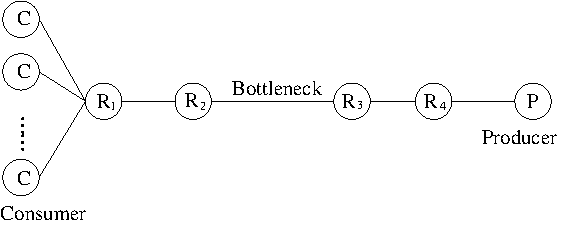
\includegraphics[width=2.5in]{bottleneck-topology.pdf}
\caption{Bottleneck topology using in simulation.}
\label{bottleneck-topology}
\end{figure}

\subsection{Stability analysis}
To choose suitable $\alpha$ and $\beta$ that make the system stable, we test under what $\alpha$ and $\beta$, the flow number can be estimated accurately. Once the flow number of the network can be accurately estimated, the Interest sending rate $R_{r}(t)$ can also be estimated accurately, then the system enters stable stage. So we choose the accuracy of estimating flow number as the stability metrics.

At the beginning, there are 10 flows in the network, and we test whether the flow number can accurately be estimated under different value of $\alpha$ and $\beta$. Fig.~\ref{fig-ab} shows that under such values the flow number can be accurately estimated. Fig.~\ref{fig-abwrong} shows that under these values the estimated flow number change greatly, which means that the system is not stable. From Fig.~\ref{fig-ab}, we can find (0.2,1.5) is the most suitable value to estimate the flow number. Under this value, we test whether the system is still stable when the system changes. We set the number of flows in the network as 5,10,15 and 20 respectively. Fig.~\ref{fig-abflownum} shows that under different situations the flow number can also be accurately estimated when $\alpha=0.2,  \beta=1.5$. That means a fixed value of $\alpha$ and $\beta$ can make the system enter stable stage even when the system's situation changes.

From Fig.~\ref{fig-abwrong}, we find that when $\alpha$ is close to 0.5, the system becomes unstable, and when it gets larger, the system becomes even more unstable. This can be explained as follows. Large $\alpha$ makes the system react too radically to increase $R_{r}(t)$ when $(C-S(t))>0$ or decrease $R_{r}(t)$ when $(C-S(t))<0$. Radical reaction will make the system difficult to converge. From Fig.~\ref{fig-ab}, we find that when $\alpha < 0.2$, the system will take longer time to accurately estimate the flow number. It is because small $\alpha$ makes the system increase or decrease $R_{r}(t)$ conservatively, and that will result in longer time to convergence. When $\beta$ is smaller than 1.5, although the system can be stable, the estimated flow number is not accurate compared with $\beta = 1.5$. It is because small $\beta$ can not drain the packets in the queue quickly enough. And that will result in inaccurate $R_{r}(t)$ and flow number.

The key point of the stability analysis is that, for $\alpha$ and $\beta$ we can choose a fixed value to make the system stable. Even when the system changes, such as the flow number, RTT and bandwidth, the fit value can also make the system keep stable. Although now we can not prove the best value by theory, it is possible to choose a stable value. In our simulation, we set $\alpha = 0.2$ and $\beta = 1.5$, according the analysis above.

\begin{figure}[t]
\centering
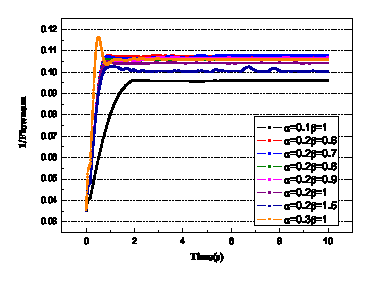
\includegraphics[width=2.5in]{ab-pic-cut.eps}
\caption{Under such $\alpha$ and $\beta$ the flow number can be accurately estimated.}
\label{fig-ab}
\end{figure}

\begin{figure}[t]
\centering
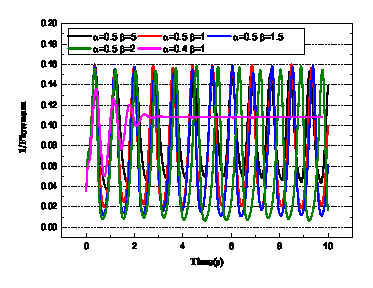
\includegraphics[width=2.5in]{abwrong-pic-cut.eps}
\caption{Under such $\alpha$ and $\beta$ the flow number can not be accurately estimated.}
\label{fig-abwrong}
\end{figure}

\begin{figure}[t]
\centering
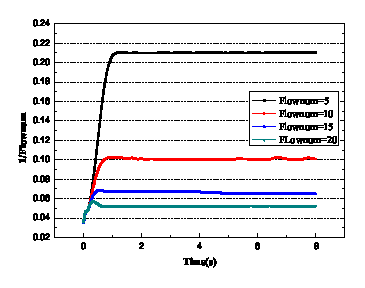
\includegraphics[width=2.5in]{abflownum-pic-cut.eps}
\caption{Stable $\alpha$ and $\beta$ can make the network stable even when network situation changes.}
\label{fig-abflownum}
\end{figure}

\subsection{The estimated flow number}

 Following Eq.~\ref{eq:flownum}, the flow number of the link can be estimated by the rate of this link. The size of Data can be estimated as the average size of the Data that goes through. Under the bottleneck network topology, at t=0, 10 flows start. At t=10 another 10 flows start. And at t=20, 10 flows finish, there are only 10 flows left. From Fig.~\ref{fig-flownum} we can see that the flow number can be accurately estimated. Even when the flow number changes, the estimation can also converge.

\begin{figure}[t]
\centering
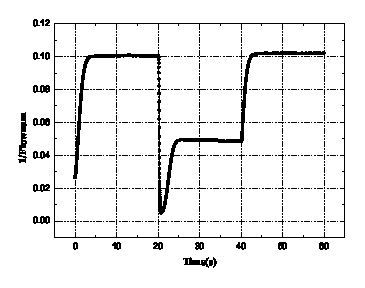
\includegraphics[width=2.5in]{flownum-pic-cut.eps}
\caption{The accuracy of estimation of flow number.}
\label{fig-flownum}
\end{figure}

\subsection{The performance of ECN-based Interest sending rate mechanism}

We use bottleneck topology to assess the ECN-based mechanism. ICP is a TCP-style Interest control protocol in NDN. The Interest sending window is passively changed according the RTT and loss of Data, following the AIMD principle\cite{ICP}. ICP-shape also follows the AIMD principle but it discards the Interest instead of Data when the routers sense congestion\cite{improveshape}. ICP-shape also sends NACK back to receiver if an Interest is shaped. NACK is a feedback information used to inform that the Interest has been discarded or there's no Data corresponding to the Interest. The consumer should retransmit the same Interest when it receives a NACK. As Fig.~\ref{fig-linkuti} shows, ICP and ICP-shape waste bandwidth because of the slow start and AIMD principle. The link utilization of ICP and ICP-shape is between 80\%-90\%. In contrast, even when the bottleneck link's bandwidth changes, the bandwidth utilization of ECN-based always closes to 100\%.

\begin{figure}[t]
	\centering
	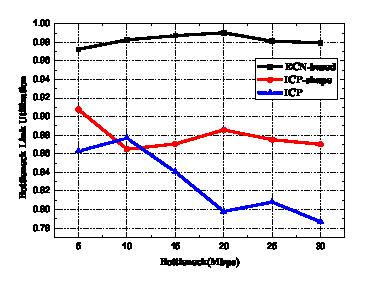
\includegraphics[width=2.5in]{utilization-pic-cut.eps}
	\caption{The bottleneck's link utilization compared with ICP and ICP-shape when change the bottleneck bandwidth.}
	\label{fig-linkuti}
\end{figure}

Because the ECN-based makes sure that the rate can't exceed the bandwidth, almost no packet (no matter Interest or Data) drops in ECN-based mechanism, as the Fig.~\ref{fig-drop} shows. ICP uses timeout as the signal to inform congestion, and timeout is caused by dropping Data. In ICP, once the link become congested, the only solution is to drop Data, so the number of dropped Data is very large. The ICP-shape shapes Interest before congestion happens, so it can reduce the number of Data needed to be dropped because of congestion. But as the delay of sending back and the difficulty of estimating the congestion, there are still some dropped Data.

\begin{figure}[t]
	\centering
	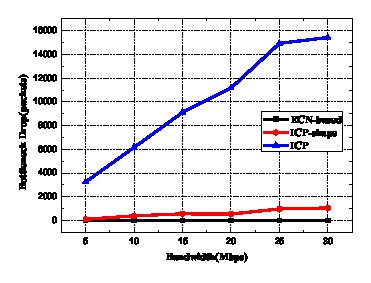
\includegraphics[width=2.5in]{drop-pic-cut.eps}
	\caption{The number of dropping packets in bottleneck compared with ICP and ICP-shape when change the bottleneck bandwidth.}
	\label{fig-drop}
\end{figure}

As Eq.~\ref{eq:updated_rt5} shows, the packets in the queue should be drained. This principle makes sure that in ECN-based, the number of packets in the queue are always close to 0, as shown in Fig.~\ref{fig-queue}.In ICP, to use the bandwidth effectively, the receivers always try to enlarge the Interest window until the Data fills up the queue and the Data is dropped, so the number of packets in the queue is largest compared with other two mechanisms. In ICP-shape, the router can shape Interest when it senses that congestion happens. So in ICP-shape, the number of queue size is less than ICP, as shown in Fig.~\ref{fig-queue}.

\begin{figure}[t]
	\centering
	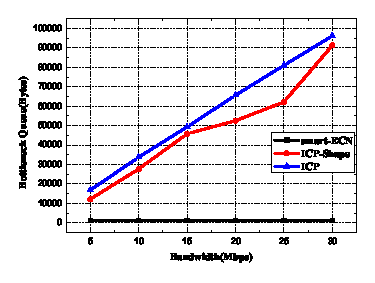
\includegraphics[width=2.5in]{queu-pic-cut.eps}
	\caption{The queuing packets in bottleneck compared with ICP and ICP-shape when change the bottleneck bandwidth.}
	\label{fig-queue}
\end{figure}

Fig.~\ref{fig-fct} shows the FCT(Flow Complete Time) of different flows. FCT in NDN is defined as the time from when receiver sends the first Interest until the receiver receives the last Data of the flow. The ECN-based mechanism's link utilization is much higher than ICP. ECN-based mechanism fairly distributes bandwidth resource to all the flows, so even the short flow can get fair bandwidth resource. No matter flows are short or long, ECN-based'FCT is much better than ICP.

\begin{figure}[t]
	\centering
	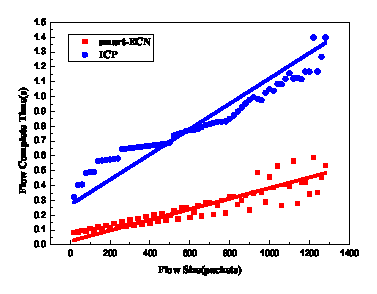
\includegraphics[width=2.5in]{fct-cut.eps}
	\caption{ECN-based's flow complete time compared with ICP.}
	\label{fig-fct}
\end{figure}

\subsection{Flow complete time compared with ICP}

We demonstrate the effectiveness of SECN(Smart forwarding with ECN-based) using mesh network topology ,as shown in Fig.~\ref{mesh-topology}. As Fig.~\ref{fig-tfct} shows, under different total bandwidth, the SECN's TFCT is much better than non-adaptive mechanism. As smart adaptive forwarding mechanism can choose the best path on the network-wide view, it's total flow complete time is even better than adaptive mechanism. The total bottleneck bandwidth refers to the sum of bottleneck bandwidth on all the available paths. Using the forwarding-assistance and route information, as shown in Fig.~\ref{fig-assistant-information}, the smart adaptive forwarding mechanism can choose the network-wide best path. The non-adaptive mechanism chooses the path by the route information, similar with TCP/IP. The non-adaptive mechanism can not change the forwarding interface according to the network condition. The adaptive mechanism chooses the best forwarding interface just by the next hop's link information. As the next hop link information can not reflect the whole path's information, the adaptive mechanism sometimes chooses a path whose later link is shared by far more flows.

\begin{figure}[t]
\centering
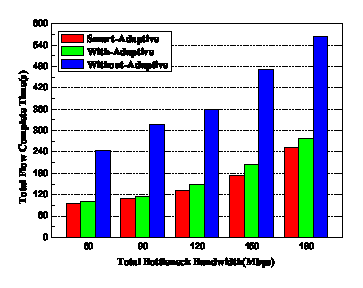
\includegraphics[width=2.5in]{adaptive-pic-cut.eps}
\caption{Total flow complete time compared with other two forwarding mechanisms.}
\label{fig-tfct}
\end{figure}



\section{Conclusion}
In conclusion, we propose a ECN congestion control and smart forwarding mechanism in NDN. Data carries the ECN information to receivers. Receivers use ECN information to adjust its Interest sending rate. Under smart forwarding mechanism, routers choose a best forwarding interface using the SDN controller's network-view information. The ECN transport mechanism can ultimately use the link utilization and reduce the dropping packets. By joining the smart forwarding and ECN transport mechanism, the whole network resource can be effective used and total flow complete time can be reduced.

The future work will be focused on the theoretical analysis of system stability. In NDN, as the in-network cache, a Data will have several providers. That will influence the ECN information carried by Data and the RTT. We want to analysis what would happen on such situation and how to make effective resolution for this.

\begin{thebibliography}{1}

\bibitem{NDN}
V. Jacobson, D. K. Smetters, J. D. Thornton, M. F. Plass, N. H. Briggs,
and R. L. Braynard, ``Networking named content," in Proceedings of ACM
CoNEXT, 2009.
\bibitem{ICP}
G. Carofiglio, M. Gallo, and L. Muscariello, ``ICP: Design and evaluation
of an interest control protocol for content-centric networking," in Proc.
1st IEEE Int��l Workshop on Emerging Design Choices in Name-Oriented
Networking, 2012.
\bibitem{Adaptive}
C. Yi, A. Afanasyev, L. Wang, B. Zhang, and L. Zhang, ``Adaptivd forwarding
in named data networking," in SIGCOMM Comput.Commun.Rev, 2012.
\bibitem{CCTCP}
L. Saino, C. Cocora, and G. Pavlou, ``CCTCP: A scalable receiver-driven
congestion control protocol for content centric networking," in Proc.IEEE ICC Int��l Conference, 2013.
\bibitem{shape}
N. Rozhnova and S. Fdida, ``An effective hop-by-hop interest shaping
mechanism for ccn communications," in Proc.1st IEEE Int��l Workshop on Emerging Design Choices in Name-Oriented Networking, 2012.
\bibitem{SDN}
A. Voellmy and J. Wang, ``Scalable software defined network controllers," in ACM SIGCOMM Computer Communication Review, 2012
\bibitem{XCP}
D. Katabi, M. Handley and C. Rohrs, ``Congestion control for high
bandwidth-delay product networks," in Proc.of ACM SIGCOMM,2002.
\bibitem{RCP}
N. Dukkipati, M. Kobayashi, R. Zhang-Shen, and N. McKeown, ``Processor
sharing flows in the internet," in IWQOS, 2006.
\bibitem{TCP}
V. Jacobson, ``Congestion avoidance and control," in SIGCOMM Comput.Commun.Rev, 1988.
\bibitem{selfish}
L. Qiu, Y. R. Yang, Y. Zhang, and S. Shenker, ``On selfish routing in internet-like environments," in Proc. of the ACM SIGCOMM,2003.
\bibitem{ndnroute}
R. Ahmed, and M. F. Bari, `` $\alpha$Route: A Name Based Routing Scheme for Information Centric Networks," in Proc. of IEEE INFOCOM 2013.
\bibitem{NDNanalysis}
S. Braun, M. Monti, M. Sifalakis and C. Tschudin, ``An empirical study of
receiver-based AIMD flow control strategies for CCN," in IEEE ICCCN,2013.
\bibitem{Flow}
S. Oueslati, J. Roberts, and N. Sbihi, ``Flow-aware Traffic Control for
a  Content -Centric Network," in IEEE INFOCOM, 2012.
\bibitem{Multipath}
G. Carofiglio, M. Gallo, and L. Muscariello, ``Multipath congestion control in content-centric networks," in IEEE INFOCOM, 2013.
\bibitem{Contug}
S. Arianfar, P. Nikander, L. Eggert, and J. Ott, ``Contug: A receiver driven transport protocol for content-centric networks," in IEEE ICNP 2010 (Poster session),2010.
\bibitem{improveshape}
Y. G. Wang, N. Rozhnova, A. Narayanan, D. Oran, and I. Rhee, ``An improved hop-by-hop interest shaper for congestion control in named data networking," in Proc. Of ACM SIGCOMM ICN, 2013.
\bibitem{ndnsimnet}
http://ndnsim.net/
\bibitem{ndnsim}
A. Afanasyev, I. Moiseenko, and L. Zhang, ``ndnSIM: NDN simulator for NS-3," in NDN, Technical Report NDN-0005, 2012.


\end{thebibliography}


% that's all folks
\end{document}


